\section{\mbox{Load-shedding} Policies}
\label{sec:ls-eval}

This section describes experiments that evaluate the use of the \sic quality metric for
\mbox{load-shedding}. Using the \sic metric, it is possible to implement \emph{semantic shedding
policies}~\cite{sem-ls} that discard tuples based on their information content.
% The \sic metric measures the amount of failure that occurred during the creation of a tuple and is thus
% an indication of the quality of the data.
These experiments evaluate a \emph{fair shedding} policy (see Section~\ref{sec:fair-shedding}), which is
designed to provide an equal allocation of system resources, with the goal of equalising the
quality of processing (\ie same \sic value) for all running queries under continuous overload.
We compare the fair shedding to a random shedding policy.
% The fair shedding policy is an implementation of the algorithm presented in
% Section~\ref{sec:fairness-algo}.
% The goal of this policy is to achieve fairness in the resource allocation for all queries running into
% the system.
% The policy strives to equalise the SCR values achieved by the result tuples of all queries.
\vspace{-15pt}
\subsection*{Fairness Comparison}
\vspace{-5pt}
This section compares the random and the fair load-shedding policies. 
The fair shedder selects the tuples to be discarded in a way that equalises the processing
degradation of all queries so that their normalised (\ie in the [0,1] interval) result SCR values are numerically
close.
The random shedder, instead, picks the tuples to be discarded at random.
Our results shows that the fair shedder always outperforms the random shedder,
achieving a higher average quality of the results (mean) and also a lower spread, measured
using a sort of dispersion metrics (IQR, Q.95-Q.05 and STD).
The experimental set-up for this set of experiments consists of 25 Emulab nodes, as described in
Table~\ref{table:machines}.
The query workload is a mix of three different queries: average, covariance and top-5, as described in
Table~\ref{table:queries}. 

Each run of the experiment compares the performance of the random and fair shedding policies, varying the
number of query partitions (\ie subqueries) for each query, while trying to maintain a similar total
number of queries. 
This means that, if the number of partitions per query increases, the total number of queries
decreases (see Table~\ref{table:partitions}). 
A larger number of subqueries distributes the load of each individual query over
a larger number of nodes, increasing the overhead due to the inter-node network communication.
The goal is to explore the effect of increasing the number of partitions for the same number of queries,
while comparing the two load-shedding policies.

Table~\ref{table:partitions} shows a breakdown of the workload characteristics for each experimental run.
The first column lists the number of subqueries that each query has been partitioned into, the second
column shows the total number of deployed queries, and the final column shows the total number of
subqueries deployed. The last row contains the data for the \emph{mixed} run, in which each query is
divided into a random number of partitions between 2 and 6.
% 
% \begin{figure}[h!]
% \centering
% 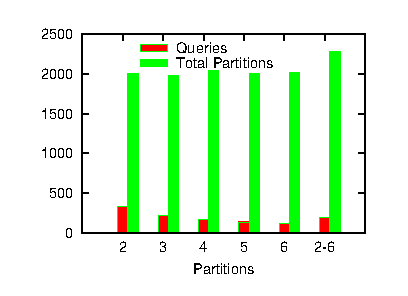
\includegraphics[width=0.6\textwidth]{img/tesi/partitions}
% \caption{Fair and random shedders comparison: IQR.}
% \label{fig:iqr}
% \end{figure}

%% --- TABLE PARTITIONS ----
\begin{table}[t]
  \centering
  \renewcommand{\arraystretch}{1.5}
  \begin{tabular}{|c|c|c|c|} 
  \hline
    %\multicolumn{4}{|c|c|c|c|}{
    \bf Partitions & \bf Queries & \bf Total Subqueries \\ 
    \hline\hline
	2 & 334 & 2004 \\
	\hline 
	3 & 220 & 1980 \\
	\hline
	4 & 170 & 2040 \\
	\hline
	5 & 134 & 2010 \\
	\hline
	6 & 112 & 2016 \\
	\hline
	2-6 & 190 & $\sim$2280 \\
    \hline
  \end{tabular}
  \caption{Workload breakdown for experiments comparing the random and fair \mbox{load-shedding}
  partitions.}
  \label{table:partitions}
\end{table}

\vspace{-10pt}
\subsection*{Statistical Measures} 
The following statistical measures are used to compare the two \mbox{load-shedding} policies. 
The first, mean, is used to evaluate the average performance of the system, while the
other three capture the dispersion of results. 
Before discussing the experimental results, we provide definitions for each of them:

\textbf{Mean:} The arithmetic mean is defined as the value obtained by summing all elements of the
sample and dividing by the total number of elements in the sample. It is used to provide an
indication of the central tendency of the data set.

\textbf{Standard deviation:} The standard deviation of a data set~\cite{std} is defined as the square
root of its variance. Variance is defined as the sum of the squared distances of each term in the
sample from the mean, divided by the total number of elements in the sample.
It shows how much variation (or dispersion) exists from the mean. A low
standard deviation indicates that the data points tend to be close to the mean, whereas a high
standard deviation indicates that the data points are spread out over a large range of values.

\textbf{Interquartile range:} The interquartile range (IQR)~\cite{upton1996understanding} is a measure of
variability based on dividing a data set into quartiles.
Quartiles divide a rank-ordered data set into four equal parts. The values that divide each part are
called the first, second and third quartiles. They are denoted by Q1, Q2, and Q3, respectively. Q1 is the
middle value in the first half of the rank-ordered data set; Q2 is the median value in the set; and Q3 is
the middle value in the second half of the rank-ordered data set. The interquartile range is equal to
Q3 minus Q1.

\textbf{Q0.95-Q0.05:} This is a measure of variability used in a similar
way to the interquartile range.
The ordered data is divided into 100 equal parts, called percentiles. Q0.95-Q0.05 captures the
spread of the middle 90\% of the ordered data values. It shows the spread
of the majority of the data values and captures a larger set of values than the IQR.

% \textbf{Median:} The median~\cite{median} is described as the numerical value separating the higher half
% of a sample, a population, or a probability distribution, from the lower half. The median of a finite list of numbers
% can be found by arranging all the observations from lowest value to highest value and picking the middle
% one. If there is an even number of observations, then there is no single middle value; the median is then
% usually defined to be the mean of the two middle values.
\subsubsection*{Experimental Results} 
The first graph, in Figure~\ref{fig:mean} shows the comparison
between the random and the fair shedding policies in terms of average quality of the delivered results.
In all the experiments, the fair shedder outperforms the random one, achieving on average results
with a higher \sic value than the random shedder. \\
The last three graphs in Figures~\ref{fig:iqr},~\ref{fig:std}~and~\ref{fig:qq} show the comparison
between the random and the fair shedding policies in terms of variability. For all the dispersion
measures used, the fair shedder achieves a lower value compared to the random shedder. This means that
the fair shedder chooses a better set of tuples to be discarded, leading to a higher mean \sic value
and a lower dispersion~of~\sic~values. 
\vspace{-10pt}
\begin{figure}[b]
\centering
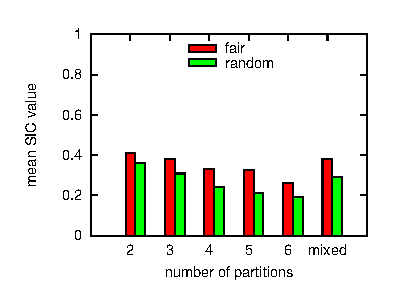
\includegraphics[width=0.55\textwidth]{img/tesi/mean}
\caption{Comparison of fair and random load shedders (MEAN).}
\label{fig:mean}
\end{figure}
\clearpage
\begin{figure}[h]
\centering
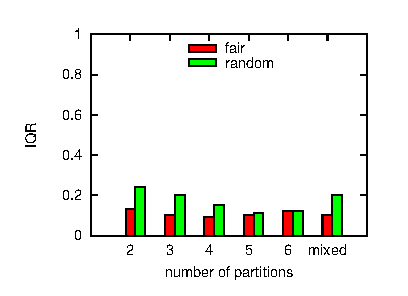
\includegraphics[width=0.55\textwidth]{img/tesi/iqr}
\caption{Comparison of fair and random load shedders (IQR).}
\label{fig:iqr}
\end{figure}
\begin{figure}[h]
\centering
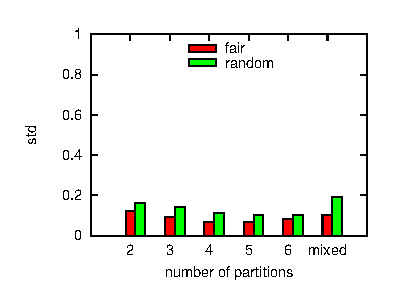
\includegraphics[width=0.55\textwidth]{img/tesi/std}
\caption{Comparison of fair and random load shedders (Standard Deviation). }
\label{fig:std}
\end{figure}
\begin{figure}[h!]
\centering
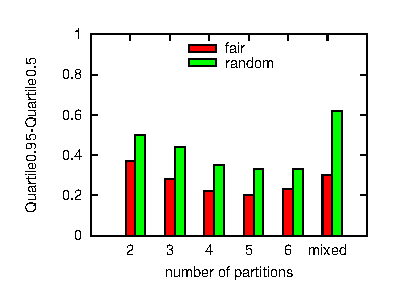
\includegraphics[width=0.55\textwidth]{img/tesi/maxmin}
\caption{Comparison of fair and random load shedders (Q0.5-Q0.95).}
\label{fig:qq}
\end{figure}
\clearpage
All experiments show a performance impact for breaking the queries into more partitions for all the analysed
measures. This is due to the higher cost of inter-node communication. A larger number of subqueries
provides a better load distribution among all the processing nodes but it also increases the total load
imposed on the system. The \emph{mean} \sic value is higher in the case of two partitions and decreases
as the number of partitions increases. The \emph{dispersion} metrics, instead, have lower values for two
partitions. Their value increases when increasing the number of subqueries.
%\clearpage

%\clearpage

%%%%%%%%%%%%%%%%%%%%%%%%%%%%%%%%%%%%%%%%%%%%%%%%%%%%%%%%%%%%%%%%%%%%%%%%%%%%%%%%%%%%%%%%%%%%%%%%%%%%%%%%%
\subsection*{Scalability of Fair Load Shedder }

The following set of experiments evaluate the scalability of the \emph{fair load shedder} in
terms of the number of nodes and queries. The aim is to observe the variation of the result \sic values
if the amount of processing resources changes. In the first set of experiments, the amount of load
remains constant, while increasing the processing resources.
Adding more nodes leads to an increase in the result \sic values because the amount of required
\mbox{load-shedding} is reduced. In the second set of experiments, the variation is in terms of
processing load, while maintaining a constant amount of processing resources. In this case, increasing
the number of deployed queries leads to a reduction of \sic values. 
% Both sets of experiments show a proportional variation of quality-of-serv ice, showing efficient
% scalability properties for the fair shedder.
Both sets of experiments are deployed on the Emulab testbed, as described in Table~\ref{table:machines}.
The processing nodes are loaded with an evenly mixed workload of
COV, AVG and TOP-5 queries, as described in Table~\ref{table:queries}.
%--------------------------------------------------------------------------------------------------------
\vspace{-10pt}
\subsubsection*{Increasing the Number of Nodes}

This set of experiments measures the scalability of the fair shedding policy in terms of
number of nodes, when varying the amount of processing
resources. Increasing the number of nodes with a fixed number of queries,
progressively reduces the overload on each processing node. The fair shedder should achieve a
proportionally better processing quality in terms of the mean \sic value. Ideally, reducing the number of
nodes by 50\% should result in the same reduction in the \sic values of the~computed~results.

Figure~\ref{fig:scalability:nodes} shows the results obtained after running the experiment on a number of
nodes varying from 9 to 24. Increasing the number of processing nodes reduces the average load
on each node and thus the need for \mbox{load-shedding}. The higher amount of available processing
resources leads to an increase in average \sic values of the output tuples. 
All dispersion measures show a reduction, which means that a better result is also achieved in terms
of the variability of the output \sic values. The value of the dispersion measures grow together with
the value of the mean. 
\begin{figure}[h!]
\centering
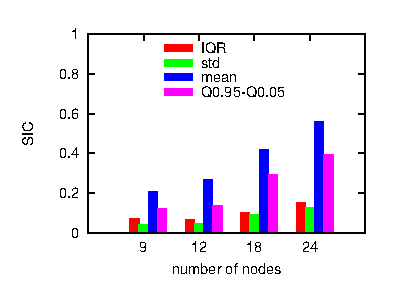
\includegraphics[width=0.55\textwidth]{img/tesi/nodes2}
\caption{Fairness for an increasing number of nodes.}
\label{fig:scalability:nodes}
\end{figure}
If the value of the mean doubles, the value of the dispersion metrics
tends to double as well because the variability range is larger. With a mean of 0.2, we can expect the
\sic values to be distributed in the interval [0,0.4], while with a mean of 0.4, we can expect the range
to be [0,0.8]. Since the range is doubled, the dispersion measures should also be doubled. What should
remain constant is the ratio between the dispersion measure and the mean, as observed this stable
ratio between the standard deviation and the mean is referred to as \emph{coefficient of
variation}~\cite{cvar}.
\vspace{-10pt}
%------------------------------------------------------------------------------------------------
\subsubsection*{Increasing the Number of Queries}

This set of experiments observes the processing quality in terms of the \sic value when varying the
number of queries (\ie increasing the load), while maintaining a constant amount of processing resources. 
The total number of nodes used in these experiments is 25 (see Table~\ref{table:machines}).
The nodes host an increasing number of queries, with an evenly mixed workload of
COV, AVG-all and TOP-5 queries (see Table~\ref{table:queries}).

Figure~\ref{fig:scalability:queries} shows the degradation in \sic values when deploying a
number of queries that varies from 180 to 1200. The results indicate that the value of all queries is
reduced proportionally to the number of queries. From the graph, it is possible to observe that the performance
of the system is not strictly linear. The slope of the descending mean \sic values changes sign, meaning
that initially the percentile reduction in the \sic value is lower than the relative increase in
the number of queries. At a certain point, this changes and the system behaviour becomes sublinear.
The next section shows how it is possible to exploit this behaviour to expose a trade-off between the
quality of results in terms of \sic values and the resource cost per query.
\begin{figure}[h!]
\centering
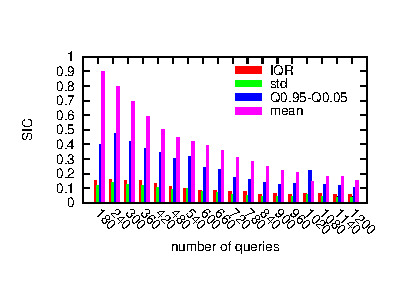
\includegraphics[width=0.7\textwidth]{img/tesi/queries_large}
\caption{Fairness for an increasing number of queries.}
\label{fig:scalability:queries}
\end{figure}
%\clearpage
% To better analyse the 
% Figure~\ref{fig:scalability:risk} shows the \emph{signal-to-noise} ratio, defined as the ratio between
% the mean \sic value and the standard deviation of the sample for all experimental runs. 
% The results show that the system performance is fairly stable, meaning that there is graceful degradation
% of the quality-of-service when increasing the processing load.
% % 
% \mnote{106: What else: try to be more verbose here as this is the main result.
% That using the SCR metric the fair shedder is able to use source data
% across queries more efficiently than the random. That similar result
% hold for different partitions. That the mixed is the most important result.}



% 
% \begin{figure}[t]
% \centering
% 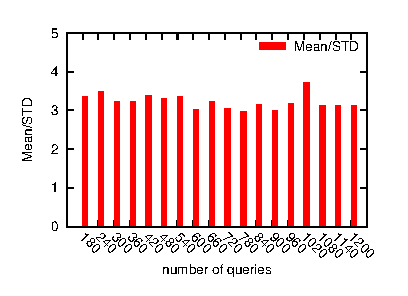
\includegraphics[width=0.6\textwidth]{img/tesi/risk}
% \caption{Stability of performance in terms of Mean/STD for increasing number of queries experiment.}
% \label{fig:scalability:risk}
% \end{figure}
%  
%\clearpage
%--------------------------------------------------------------------------------------------------------

